\documentclass[a4paper,12pt,oneside]{book}
\usepackage[utf8]{inputenc}
\title{}
\author{Rachel Morris}
\date{\today}

\usepackage{rachwidgets}
\usepackage{fancyhdr}
\usepackage{lastpage}
\usepackage{boxedminipage}
\usepackage{fancyvrb}

\newcommand{\laClass}{CS 250\ }
\newcommand{\laSemester}{Fall 2017\ }
\newcommand{\laLab}{Project 2: Stacks and Queues\ }

\pagestyle{fancy}
\fancyhf{}
\lhead{\laClass}
\chead{\laSemester}
\rhead{\laLab}
\rfoot{\thepage\ of \pageref{LastPage}}
\lfoot{By Rachel Morris, \footnotesize last updated \today}

\renewcommand{\headrulewidth}{2pt}
\renewcommand{\footrulewidth}{1pt}

\begin{document}

    \chapter*{\laLab} \stepcounter{chapter}

        \section{Information}
            \paragraph{ Topics: } Stacks, Queues, LinkedList, Templates
            \paragraph{ Turn in: } All source files (.cpp and .hpp).
            \paragraph{ Starter files: } Download on GitHub or D2L.

        \subsection{About}

% ----------------------------------------------------------------------
% ----------------------------------------------------------------------
% ----------------------------------------------------------------------

\renewcommand*\DTstylecomment{\rmfamily\color{green}\textsc}

\begin{framed}
\dirtree{%
.1 Project 2 - Stacks and Queues/.
.2 main{.}cpp
    \dots{} \begin{minipage}[t]{5cm} Contains main() \end{minipage}.
.2 AirTravelSimulator{.}hpp
    \dots{} \begin{minipage}[t]{5cm} Contains main program code \end{minipage}.
.2 AirTravelSimulator{.}cpp.
.2 Airplane{.}hpp
    \dots{} \begin{minipage}[t]{5cm} The virtual Airplane \end{minipage}.
.2 Airplane{.}cpp.
.2 Airport{.}hpp
    \dots{} \begin{minipage}[t]{5cm} The virtual Airport \end{minipage}.
.2 Airport{.}cpp.
.2 Traveller{.}hpp
    \dots{} \begin{minipage}[t]{5cm} Traveller structure \end{minipage}.
.2 TravelManager{.}hpp
    \dots{} \begin{minipage}[t]{5cm} Contains all travellers \end{minipage}.
.2 States{.}hpp
    \dots{} \begin{minipage}[t]{10cm} Different program states \end{minipage}.
.2 names{.}txt
    \dots{} \begin{minipage}[t]{10cm} Data file with traveller names \end{minipage}.
.2 DataStructures/
    \dots{} \begin{minipage}[t]{7cm}
        Data structures are stored here
    \end{minipage}.
.3 LinkedList{.}hpp.
.3 Queue{.}hpp.
.3 Stack{.}hpp.
.2 docs/html/index{.}html
    \dots{} \begin{minipage}[t]{5cm}
        The documentation files
    \end{minipage}.
}
\end{framed}

This program does not have any unit tests associated with it.

    \newpage

    \subsection{Documentation}

    For this program, documentation has been auto-generated using \textit{doxygen}.
    The documentation is also available as comments in the source code, so
    you can read the function notes in either place.

    To access the documentation outside of the code, go to the \textbf{docs}
    folder, then the \textbf{html} folder.

    \begin{figure}[h]
        \center
        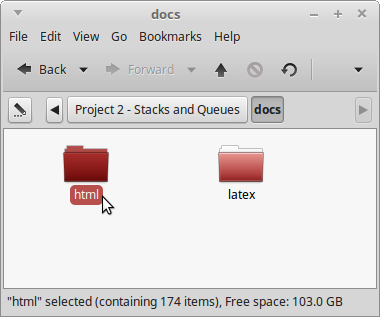
\includegraphics[width=6cm]{images/project2-docsfolder.png}
        \caption{Inside the docs folder}
    \end{figure}

    Then, open \textbf{index.html}. You can click on the \textbf{Classes}
    tab to view a list of all classes in the program, and clicking on
    a class will take you to its documentation page, which includes the
    descriptions of functionality you will need to implement.
    \textbf{All of the functions' documentation is in the doxygen page.}

    \begin{figure}[h]
        \center
        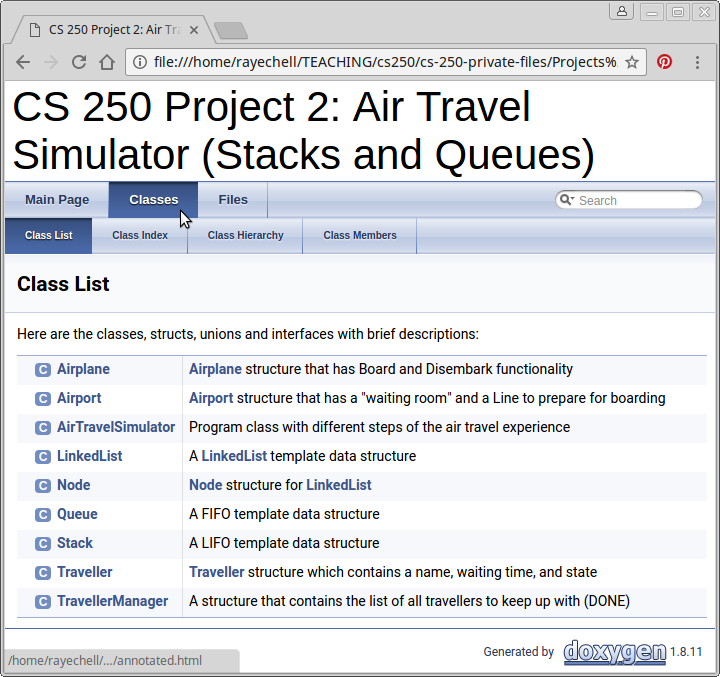
\includegraphics[height=8cm]{images/project2-classlist.png}
        \caption{The list of classes in the documentation}
    \end{figure}

    \begin{figure}[h]
        \center
        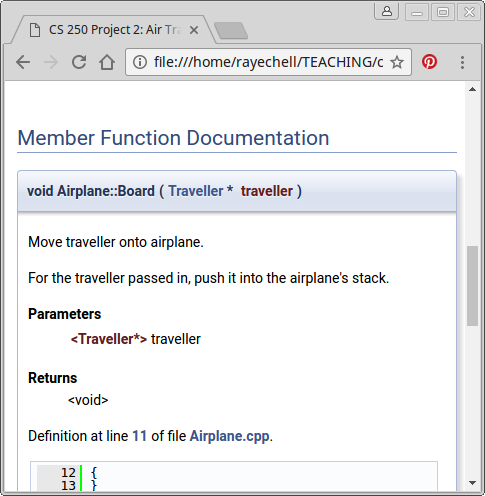
\includegraphics[height=8cm]{images/project2-functions.png}
        \caption{A function's documentation}
    \end{figure}
    
    \subsection{Adding on to Airport and Airplane}

    You will need to add the following members to the Airport and Airplane classes:
    
    \begin{itemize}
        \item Airport: Add a Stack of Traveller pointers as a member variable
        \item Airplane: Add a Queue of Traveller pointers as a member variable
    \end{itemize}
    
% ----------------------------------------------------------------------
% ----------------------------------------------------------------------
% ----------------------------------------------------------------------
    \chapter*{Grading Breakdown}

    \textbf{Features}
    
    \begin{center}
        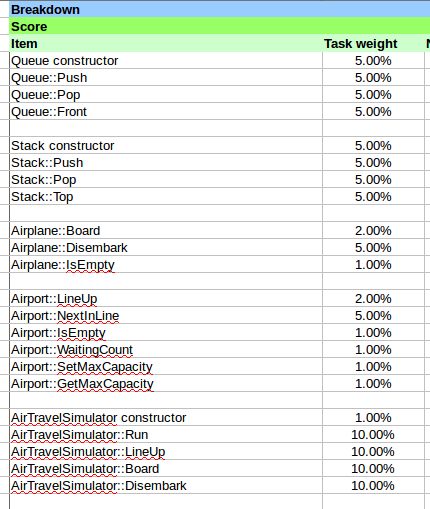
\includegraphics[height=14.5cm]{images/gradesheet-project2.png}
    \end{center}

    \newpage
    \textbf{Penalties}
    
    \begin{center}
        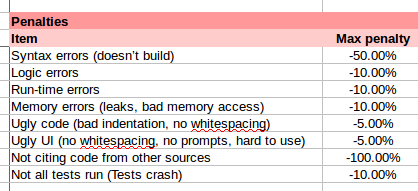
\includegraphics[width=12cm]{images/gradesheet-project2-penalties.png}
    \end{center}


\end{document}









